\chapter{Topological vector spaces over a valued division ring}

\section{TOPOLOGICAL VECTOR SPACES}

\subsection{Definition of a topological vector space}

DEFINITION 1. --- Given a topological division ring K (GT, III, § 6.7) and a set E such that E has

\(1^{\circ}\) the structure of a left vector space on \(\mathbf{K}\) ;

\(2^{\mathrm{o}}\) a topology compatible with the structure of the additive group of E (GT, III,

§ 1.1) and satisfying in addition the following axiom :

(EVT) the mapping \((\lambda, x) \mapsto \lambda x\) of \(\mathbf{K} \times \mathbf{E}\) in \(\mathbf{E}\) is continuous,

then E is called a left topological vector space over (or on) K.

It is equivalent to saying that E is a topological left K-module (GT, III, § 6.6).

A left vector space structure relative to K and a given topology on a set E, are said to be compatible if the topology and the additive group structure of E are compatible and if, in addition, the axiom (EVT) is valid. This is the same as saying that the two mappings \((x, y) \mapsto x + y\) and \((\lambda, x) \mapsto \lambda x\) of \(E \times E\) and of \(K \times E\) , respectively, in E are continuous, for then the mapping \(x \mapsto -x = (-1)x\) , is continuous and the topology of E is compatible with its additive group structure.

If \(\mathbf{E}\) is a left topological vector space over \(\mathbf{K}\) , we say that \(\mathbf{E}\) provided only with its vector space structure, underlies the topological vector space \(\mathbf{E}\) .

compatible with the vector space structure of E on R. For, let \(u_{0}\) be a point of E, let H be a compact subset of X and \(\varepsilon\) be an arbitrary strictly positive number. The real-valued function \(u_{0}\) is bounded in H; let \(a = \sup_{t \in H} |u_{0}(t)|\) ; if u is any point of E then for all \(t \in H\)

\[
\left| \lambda u (t) - \lambda_ {0} u _ {0} (t) \right| \leqslant | \lambda |. \left| u (t) - u _ {0} (t) \right| + a \left| \lambda - \lambda_ {0} \right|.
\]

Hence, if \(|\lambda - \lambda_0| \leqslant \varepsilon\) and \(|u(t) - u_0(t)| \leqslant \varepsilon\) for all \(t \in \mathbf{H}\) , then for \(t \in \mathbf{H}\) , \(|\lambda u(t) - \lambda_0 u_0(t)| \leqslant \varepsilon (\varepsilon + |\lambda_0| + a)\) , which shows that the axiom (EVT) is satisfied; similarly it can be verified that the compact convergence topology is compatible with the additive group structure of \(\mathbf{E}\) .

On the other hand, if X is not compact, the uniform convergence topology (in X) is not necessarily compatible with the vector space structure of E; for example if X = R and if \(u_{0}\) is an unbounded continuous function in R, then the mapping \(\lambda \mapsto \lambda u_{0}\) of R in E is not continuous in the uniform convergence topology on E.

\begin{enumerate}
\def\labelenumi{\arabic{enumi})}
\setcounter{enumi}{4}
\tightlist
\item
  Let E be a vector space of finite dimension n over a topological division ring K; there exists an isomorphism \(u:K_{s}^{n}\to E\) of vector K-spaces and moreover, if v is a second isomorphism of \(K_{s}^{n}\) on E, then we can write \(v=u\circ f\) , where f is an automorphism of the vector K-space \(K_{s}^{n}\) . Consider, on \(K_{s}^{n}\) , the product topology that is compatible with its vector space structure (Example 3); since every linear mapping of \(K_{s}^{n}\) in itself is continuous for this topology, every automorphism of the vector space \(K_{s}^{n}\) is bicontinuous. Hence, if we transfer the product topology of \(K_{s}^{n}\) to E, by means of any isomorphism whatever of \(K_{s}^{n}\) on E, the topology obtained on E is independent of the particular isomorphism used; we call it the canonical topology on E; we shall characterize it differently (I, § 1.3) when K is a non-discrete complete division ring with a valuation. Every linear mapping of E in a topological vector space over K is continuous for the canonical topology on E.
\end{enumerate}

In the same way as in def. 1, a right topological vector space over K, a topological division ring, can be defined; but every right vector space on K can be considered as a left vector space on the division ring \(K^{0}\) opposite to K (A, II, § 1.1) and the topology of K is compatible with the structure of the division ring \(K^{0}\) . For this reason we usually consider only left topological vector spaces; when we speak of «topological vector space» without qualification, it is to be understood that we refer to a left vector space.

If \(K'\) is a sub-division ring of K, and E a topological vector space over K, then it is clear that the topology of E is still compatible with the vector space structure of E relative to \(K'\) , obtained by restricting the field of scalars to \(K'\) ; we say that the topological vector space on \(K'\) , obtained by this procedure, underlies the topological vector space E on K.

In order that a topological vector space E be Hausdorff, it is necessary and sufficient that for all \(x \neq 0\) of E, there exists a neighbourhood of 0 not containing x (GT, III, § 1.2).

Consider a topology, on a vector space E over a topological division ring K, that is compatible with the additive group structure of E. Because of the identity

\[
\lambda x - \lambda_ {0} x _ {0} = (\lambda - \lambda_ {0}) x _ {0} + \lambda_ {0} (x - x _ {0}) + (\lambda - \lambda_ {0}) (x - x _ {0})
\]

axiom (EVT) is equivalent to the following system of three axioms.

(EVT') For all \(x_0 \in \mathrm{E}\) , the mapping \(\lambda \mapsto \lambda x_0\) is continuous at \(\lambda = 0\) .

(EVT \(_{II}\) ) For all \(\lambda_{0}\in K\) , the mapping \(x\mapsto\lambda_{0}x\) is continuous at x=0.

\((\mathrm{EVT}_{\mathrm{III}}^{\prime})\) The mapping \((\lambda, x) \mapsto \lambda x\) is continuous at \((0, 0)\) .

In particular :

PROPOSITION 1. --- For all \(\alpha \in \mathbf{K}\) and every point \(b \in \mathbf{E}\) , the mapping \(x \mapsto \alpha x + b\) of \(\mathbf{E}\) in itself is continuous. Further, if \(\alpha \neq 0\) , this mapping is a homeomorphism of \(\mathbf{E}\) on itself.

The second part of the proposition is a result of the fact that if \(\alpha \neq 0\) , then \(x \mapsto \alpha^{-1}x - \alpha^{-1}b\) is the inverse mapping of \(x \mapsto \alpha x + b\) .

COROLLARY. --- If A is an open (resp. closed) set in E, then \(\alpha A\) is open (resp. closed) in E for every \(\alpha \neq 0\) in K.

Let E and F be two topological vector spaces on the same topological division ring K. A bijection f of E on F is an isomorphism of the topological vector space E on the topological vector space F if and only if f is linear and bicontinuous. In particular, if \(\gamma \neq 0\) belongs to the centre of K, the homothety \(x \mapsto \gamma x\) is an automorphism of the topological vector space structure of E.

\subsection{Normed spaces on a valued division ring}

Recall (GT, IX, § 3.2) that an absolute value on a division ring K is a mapping \(\xi \mapsto |\xi|\) of K in \(\mathbf{R}_{+}\) , such that \(|\xi| = 0\) if, and only if, \(\xi = 0\) , and that \(|\xi \eta| = |\xi| \cdot |\eta|\) , and \(|\xi + \eta| \leqslant |\xi| + |\eta|\) ; an absolute value defines a distance \(|\xi - \eta|\) on K, and hence a Hausdorff topology compatible with the division ring structure of K. If \(|\xi| = 1\) for all \(\xi \neq 0\) , the absolute value is called improper, and the topology that it defines on K is the discrete topology; if, on the other hand, there exists \(\alpha \neq 0\) in K such that \(|\alpha| \neq 1\) , then there exists \(\beta \neq 0\) in K such that \(|\beta| < 1\) (it is sufficient to take \(\beta = \alpha\) or \(\beta = \alpha^{-1}\) ), and the sequence \((\beta^n)_{n \geqslant 1}\) converges to 0, thus the topology of K is not discrete.

We recall on the other hand (GT, IX, § 3.3) that if E is a vector space on a non-discrete valued division ring K then a norm on E is a mapping \(x \mapsto \|x\|\) of E in \(\mathbf{R}_{+}\) , such that \(\|x\| = 0\) if, and only if, \(x = 0\) , and such that \(\| \lambda x \| = |\lambda| \cdot \| x\|\) for every scalar \(\lambda \in \mathbf{K}\) , and \(\|x + y\| \leqslant \|x\| + \|y\|\) . A distance \(\|x - y\|\) , is defined on E by the norm, and hence a topology that is compatible with the vector space structure of E (loc. cit.). Unless the contrary is expressly stated, a normed space is considered in terms of the structure of the topological vector space defined by its norm. The normed spaces are among the most important of topological vector spaces.

It is known (GT, IX, § 3.3) that two distinct norms on E can define the same topology on E; for this it is necessary and sufficient that the two norms be equivalent (loc. cit.). The structure of normed spaces is thus richer than the structure of topological vector spaces; if E and F are two normed spaces one must be careful to distinguish between the idea of isomorphism of the normed space structure of E with that of F, and the idea of isomorphism of the topological vector space structure of E with that of F.

Example. --- Let I be an arbitrary set of indices; it is known (GT, X, § 3.2) that a norm \(\|x\|\) can be defined, on the set of bounded mappings \(x = (\xi_{\mathfrak{t}})\) of I in K, \(\mathcal{B}(\mathrm{I};\mathrm{K})\) (also written \(\mathcal{B}_{\mathrm{K}}(\mathrm{I})\) or \(\ell_{\mathrm{K}}^{\infty}(\mathrm{I})\) ), by \(\|x\| = \sup_{\mathfrak{t}\in \mathrm{I}}|\xi_{\mathfrak{t}}|\) . When I is a topological space, the set of bounded, continuous mappings of I in K is a closed subspace of the space \(\mathcal{B}(\mathrm{I};\mathrm{K})\) (GT, X, § 3.1, cor. 2). Another subspace of \(\mathcal{B}(\mathrm{I};\mathrm{K})\) is the set \(\ell_{\mathrm{K}}^{1}(\mathrm{I})\) of absolutely summable families \(x = (\xi_{\mathfrak{t}})\) (GT, X, § 3.6); we can define on this subspace another norm \(\|x\|_1 = \sum_{\mathfrak{t}\in \mathrm{I}}|\xi_{\mathfrak{t}}|\) , that in general is not equivalent to the norm \(\|x\| = \sup_{\mathfrak{t}\in \mathrm{I}}|\xi_{\mathfrak{t}}|\) (I, p.~23, exerc. 6); when considering \(\ell_{\mathrm{K}}^{1}(\mathrm{I})\) as a normed space, without specifying its norm, it is always the norm \(\|x\|\) , that is meant. We write \(\mathcal{B}(\mathrm{I})\) and \(\ell^1 (\mathrm{I})\) in place of \(\mathcal{B}(\mathrm{I};\mathbf{R})\) and \(\ell_{\mathbf{R}}^{1}(\mathrm{I})\) .

\subsection{Vector subspaces and quotient spaces of a topological vector space; products of topological vector spaces; topological direct sums of subspaces}

Everything that has been said for topological modules (GT, III, § 6.6) applies in particular to topological vector spaces. If M is a vector subspace of a topological vector space E, the topology induced on M by that of E is compatible with the vector space structure of M, and the closure \(\overline{M}\) of M in E is a vector subspace of E. The quotient topology of that of E by M is compatible with the vector space structure of E/M.

If E is a topological vector space, the closure N of \(\{0\}\) in E (intersection of neighbourhoods of 0) is a closed vector subspace of E; the quotient vector subspace E/N, which is necessarily Hausdorff whether E is or not, is called the Hausdorff vector space associated with E.

Let \((\mathrm{E}_{\iota})_{\iota \in I}\) be a family of topological vector spaces over the same topological division ring K, and let E be the product vector space of the \(E_{\iota}\) . The product topology of the topologies of the \(E_{\iota}\) is compatible with the vector space structure of E. In the product space E, the subspace F, the direct sum of the \(E_{\iota}\) is everywhere dense (GT, III, § 2.9, prop. 25).

For certain types of topological vector spaces on the field \(\mathbf{R}\) or the field \(\mathbf{C}\) we define (in II, p.~29) a topology on the direct sum of a family \((\mathrm{E}_{\mathrm{t}})\) of topological vector spaces that is, in general, distinct from the topology induced by the product topology of the \(\mathrm{E}_{\mathrm{t}}\) .

Everything that has been said on the finite direct sums of stable subgroups of topological groups with operators (GT, III, §6.2) applies to topological vector spaces, replacing « stable subgroup » throughout by « vector subspace ».

Remark. --- Given a closed vector subspace M of a Hausdorff topological vector space E, it is not necessarily the case that there exists an (algebraic) complementary vector subspace to M that is closed in E (even if E is a normed space; cf.~IV, p.~55, exerc. 16 (c)); a fortiori there does not necessarily exist a topological complement of M in E (cf.~I, p.~26, exerc. 8). However we shall see in § 2 that when K is a non-discrete valued division ring, then every closed subspace M of E, with finite codimension, does have a topological complement in E (I, p.~14, prop. 3).

\subsection{Uniform structure and completion of a topological vector space}

Since the topology of the topological vector space E is compatible with the additive group structure on E, it defines a uniform structure on E (GT, III, § 3); when we speak of the uniform structure of a topological vector space we always mean this structure unless the contrary is expressly stated. Every continuous linear mapping of a topological vector space E in a topological vector space F is uniformly continuous (GT, III, § 3.1, prop. 3); every mapping of E in itself of the form \(x \mapsto ax + b\) is uniformly continuous. An equicontinuous set of linear mappings of E in F is uniformly equicontinuous (GT, X, § 2.2, prop. 5).

Remarks. --- 1) If B is a precompact set of K, then for every neighbourhood V of 0 in E, there is a neighbourhood U of 0 in E such that BU ⊂ V. For, if W is a neighbourhood of 0 in E such that W + W ⊂ V; then from (EVT \(_{III}\) ) there is a neighbourhood T \(_{0}\) of 0 in K and a neighbourhood U \(_{0}\) of 0 in E such that T \(_{0}\) U \(_{0}\) ⊂ W. As B is precompact, there are finitely many points \(\lambda_{i} \in \mathbf{B}\) ( \(1 \leqslant i \leqslant n\) ) such that the \(\lambda_{i} + T_{0}\) cover B; from (EVT \(_{II}\) ) it follows that there is a neighbourhood U ⊂ U \(_{0}\) of 0 in E, such that \(\lambda_{i}\) U ⊂ W for all i; clearly U has the required properties. In a similar manner (using (EVT \(_{I}\) ) instead of (EVT \(_{II}\) )) it can be shown that if H is a precompact set of E, then for every neighbourhood V of 0 in E, there exists a neighbourhood T of 0 in K such that TH ⊂ V.

\begin{enumerate}
\def\labelenumi{\arabic{enumi})}
\setcounter{enumi}{1}
\tightlist
\item
  From 1) it follows that, if B is a precompact set of K and H is a precompact set of E, then the mapping \((\lambda, x) \mapsto \lambda x\) restricted to \(\mathbf{B} \times \mathbf{H}\) is uniformly continuous. For, if V is a neighbourhood of 0 in E then there are neighbourhoods T of 0 in K, and U of 0 in E such that \(\mathrm{TH} + \mathrm{BU} \subset \mathrm{V}\) . Since we can write \(\lambda x - \lambda' x' = (\lambda - \lambda') x + \lambda'(x - x')\) , we see that for \(\lambda, \lambda'\) in B, \(x, x'\) in H, \(\lambda - \lambda' \in \mathrm{T}\) and \(x - x' \in \mathrm{U}\) , we have \(\lambda x - \lambda' x' \in \mathrm{V}\) , which proves our assertion.
\end{enumerate}

A topological vector space is called complete if, considering its uniform structure, it is a complete uniform space.

DEFINITION 2. --- A complete normed space on a non-discrete valued division ring is called a Banach space.

Examples. --- If K is a non-discrete valued division ring then the space \(\mathcal{B}(\mathrm{I};\mathrm{K})\) (I, p.~4, Example) is complete (GT, X, § 3.1, cor. 1). This is also true for the space \(\ell_{\mathbf{K}}^{1}(\mathrm{I})\) (I, p.~4, Example) with the norm \(\| x\| _1 = \sum_{\iota \in \mathrm{I}}|\xi_\iota |:\) for, if \(x_{n}\) is a Cauchy sequence in this space and \(x_{n} = (\xi_{n\iota})_{\iota \in \mathrm{I}}\) , then for all \(\iota \in \mathrm{I}\)

\[
\left| \xi_ {m\iota} - \xi_ {n\iota} \right| \leqslant \left\| x _ {m} - x _ {n} \right\| _ {1};
\]

thus, for each \(\iota \in I\) , the sequence \((\xi_{n\iota})_{n\geqslant 1}\) converges to a limit \(\xi_{\iota}\) in K. Further, for each finite subset J of I

\[
\sum_ {\iota \in J} | \xi_ {m\iota} - \xi_ {n\iota} | \leqslant \| x _ {m} - x _ {n} \| _ {1};
\]

and it follows immediately that there exists a constant \(a > 0\) , independent of J, \(m, n\) such that \(\sum_{\iota \in \mathbf{J}} |\xi_{m\iota} - \xi_{n\iota}| \leqslant a\) . Letting \(m\) tend to \(+\infty\) , we deduce \(\sum_{\iota \in \mathbf{J}} |\xi_{\iota} - \xi_{n\iota}| \leqslant a\) from which \(\sum_{\iota \in \mathbf{I}} |\xi_{\iota}| \leqslant a + \| x_n\|_1\) , which shows that \(z = (\xi_{\iota})_{\iota \in \mathbf{I}}\) belongs to \(\ell_{\mathbf{K}}^1 (\mathbf{I})\) ; further, for all \(\varepsilon > 0\) , there exists \(n_0\) such that for \(n \geqslant n_0\) and for every finite set J of I, we have \(\sum_{\iota \in \mathbf{J}} |\xi_{\iota} - \xi_{n\iota}| \leqslant \varepsilon\) ; passing to the limit with respect to the directed set of finite subsets of I, we see that \(\| z - x_n\| _1\leqslant \varepsilon\) for \(n\geqslant n_0\) , which shows that \(z\) is the limit of the sequence \((x_{n})\) in the normed space \(\ell_{\mathbf{K}}^{1}(\mathrm{I})\)

Let K be a Hausdorff topological division ring, E a topological vector space on K and suppose that the completed ring \(\hat{K}\) is a division ring (this is so when K is a valued division ring, GT, IX, § 3.3) then the Hausdorff completion \(\hat{E}\) of E carries the structure of a complete topological vector space on \(\hat{K}\) (GT, III, § 6.5); we say that \(\hat{E}\) , with this structure, is the Hausdorff completion of the topological vector space E, or simply the completion of E when E is Hausdorff.

\subsection{Neighbourhoods of the origin in a topological vector space over a valued division ring}

DEFINITION 3. --- Let K be a valued division ring and E a left vector space over K; we say that a subset M of E is balanced if, for all \(x \in M\) and all \(\lambda \in K\) such that \(|\lambda| \leqslant 1\) , it is true that \(\lambda x \in M\) (or in other words if \(\lambda M \subset M\) when \(|\lambda| \leqslant 1\) ).

PROPOSITION 2. --- In a topological vector space E over a valued division ring K, the closure of a balanced set M, is a balanced set.

If B is the set of \(\xi\in K\) with \(|\xi|\leqslant1\) ; then B is closed in K. But \(B\times M\) is mapped into M by the continuous mapping \((\lambda,x)\mapsto\lambda x\) ; and therefore \(B\times\overline{M}\) is mapped into \(\overline{M}\) (GT, I, §2.1, th. 1) which proves that \(\overline{M}\) is balanced.

When M is an arbitrary set in the vector space E over a valued division ring K, the set \(M_{1}\) of the \(\lambda x\) with \(x \in M\) and \(\lambda \in K\) such that \(|\lambda| \leqslant 1\) , is clearly the smallest balanced set containing M; \(M_{1}\) is called the balanced envelope of M.

PROPOSITION 3. --- Let K be a valued locally compact and non-discrete division ring and E be a Hausdorff topological vector space (resp. a topological vector space) over K. For every compact (resp. precompact) set H in E, the balanced envelope of H is compact (resp. precompact).

If B denotes the ball \(|\xi| \leqslant 1\) in K, the balanced envelope of H is \(H_{1}\) , the image of \(B \times H\) under the continuous mapping \(m: (\lambda, x) \mapsto \lambda x\) . If E is Hausdorff, if B is compact and if H is compact then so is \(B \times H\) and therefore \(H_{1}\) . If H is precompact the restriction of m to \(B \times H\) is uniformly continuous (I, p.~5, Remark 2) and as \(B \times H\) is precompact, so also is its image under m (GT, II, § 4.2, prop. 2).

Note that the balanced envelope of a closed set is not necessarily closed. For example, in \(\mathbf{R}^2\) , the balanced envelope of the hyperbola defined by the equation \(xy = 1\) is not closed.

The union of a family of balanced sets in E is balanced, which implies that for every set M of E there is a largest balanced subset N of M called the balanced core of M; also N is not empty if and only if \(0 \in M\) . To say that \(x \in N\) means that for all \(\lambda \in K\) such that \(|\lambda| \leqslant 1\) , we have \(\lambda x \in M\) , or again (if \(0 \in M\) ) that, for all \(\mu \in K\) with \(|\mu| \geqslant 1\) , we have \(x \in \mu M\) . If \(0 \in M\) , the balanced core N of M is therefore the intersection \(\bigcap_{|\mu| \geqslant 1} \mu M\) . This shows in particular that if M is closed, so also is N.

DEFINITION 4. --- Let K be a non-discrete valued division ring and E be a left vector space on K with two subsets A and B. We say that A absorbs B if there exists \(\alpha > 0\) such that \(\lambda A \supset B\) for every \(\lambda \in K\) with \(|\lambda| \geqslant \alpha\) (or equivalently if \(\mu B \subset A\) for \(\mu \neq 0\) and \(|\mu| \leqslant \alpha^{-1}\) ). A set A of E is called absorbent if it absorbs every set consisting of a single point.

Let A be a balanced set of E; for it to absorb a set B of E it is sufficient that there exists \(\lambda \neq 0\) such that \(\lambda A \supset B\) ; in fact, for \(|\mu| \geqslant |\lambda|\) , we have \(\lambda A = (\lambda \mu^{-1}) \mu A\) , and as \(\mu A\) is balanced and \(|\lambda \mu^{-1}| \leqslant 1\) , it follows that \(\lambda A \subset \mu A\) , and thus \(B \subset \mu A\) . In particular for a balanced set A of E to be absorbent, it is necessary and sufficient that for every \(x \in E\) , there exists \(\lambda \neq 0\) in K such that \(\lambda x \in A\) . Every absorbent set of E generates the vector space E. Every finite intersection of absorbent sets is an absorbent set.

PROPOSITION 4. --- In a topological vector space E on a non-discrete valued division ring K there exists a fundamental system \(\mathfrak{B}\) of closed neighbourhoods of 0 such that :

\((\mathrm{EV}_{\mathrm{I}})\) Every set \(\mathbf{V}\in \mathfrak{B}\) is balanced and absorbent.

(EV \(_{II}\) ) For every V \(\in\) B and \(\lambda \neq 0\) in K, we have \(\lambda\) V \(\in\) B (invariance of B under homotheties of non zero ratio).

\((\mathrm{EV}_{\mathrm{III}})\) For every \(\mathbf{V}\in \mathfrak{B}\) , there exists \(\mathbf{W}\in \mathfrak{B}\) such that \(\mathbf{W} + \mathbf{W}\subset \mathbf{V}\) .

Conversely, let E be a vector space on K, and let V be a filter base on E satisfying the conditions \((\mathrm{EV}_{\mathrm{I}})\) , \((\mathrm{EV}_{\mathrm{II}})\) and \((\mathrm{EV}_{\mathrm{III}})\) . Then there exists a topology (and it is unique) on E, compatible with the vector space structure of E, and for which V is a fundamental system of neighbourhoods of 0.

By axiom \((\mathrm{EVT}_{\mathrm{III}}^{\prime})\) we show firstly that the balanced core, \(V_{1}\) , of V, a neighbourhood of 0, is itself a neighbourhood of 0. For there exist \(\alpha > 0\) and a neighbourhood W of 0 such that, if \(|\lambda| \leqslant \alpha\) and \(x \in W\) , then \(\lambda x \in V\) . Since K is non-discrete, there exists \(\mu \neq 0\) in K with \(|\mu| \leqslant \alpha\) and \(\mu W\) is a neighbourhood of 0 for which \(\mu W \subset V\) . Also if \(v \in K\) and \(|v| \leqslant 1\) then \(|v\mu| \leqslant \alpha\) and thus \(v\mu W \supset V\) . Hence \(\mu W \supset V_{1}\) and \(V_{1}\) is a neighbourhood of 0. Also as V is closed so also \(V_{1}\) is closed. Thus the set B of closed balanced neighbourhoods of 0 form a fundamental system of neighbourhoods of 0 in E. By \((\mathrm{EVT}_{\mathrm{I}}^{\prime})\) every neighbourhood of 0 is absorbent; furthermore B satisfies \((\mathrm{EV}_{\mathrm{II}})\) (cf.~I, p.~3, cor.); finally, because of the continuity of \((x, y) \mapsto x + y\) at the point \((0, 0)\) , every fundamental system of neighbourhoods of 0 in E satisfies \((\mathrm{EV}_{\mathrm{III}})\) . The set B satisfies the conditions of the proposition.

Now let E be a vector space over K, and V be a filter base on E satisfying \((\mathrm{EV}_{\mathrm{I}})\) , \((\mathrm{EV}_{\mathrm{II}})\) and \((\mathrm{EV}_{\mathrm{III}})\) . The axiom \((\mathrm{EV}_{\mathrm{I}})\) shows firstly that for all \(V \in V\) , we have -V = V and \(0 \in V\) ; these relations and the axiom \((\mathrm{EV}_{\mathrm{III}})\) show that V is a fundamental system of neighbourhoods of 0, for a topology on E compatible with the additive group structure of E (GT, III, § 1.2). On the other hand the axioms (EVT \(_{I}\) ), (EVT \(_{II}\) ) and (EVT \(_{III}\) ) are immediate consequences of (EV \(_{I}\) ) and (EV \(_{II}\) ), thus the topology defined above satisfies the axiom (EVT), and the proposition is proved.

Remarks. --- 1) In a normed space on a non-discrete valued division ring the set of open balls (resp. closed balls) with centre 0 is a fundamental system of neighbourhoods of 0 which satisfy the conditions \((\mathrm{EV}_{\mathrm{I}})\) , \((\mathrm{EV}_{\mathrm{II}})\) and \((\mathrm{EV}_{\mathrm{III}})\) .

\begin{enumerate}
\def\labelenumi{\arabic{enumi})}
\setcounter{enumi}{1}
\tightlist
\item
  When the division ring of scalars \(\mathbf{K}\) is the field \(\mathbf{R}\) or the field \(\mathbf{C}\) , every filter base \(\mathfrak{B}\) on \(\mathbf{E}\) which satisfies just the two axioms \((\mathrm{EV}_{\mathbf{I}})\) and \((\mathrm{EV}_{\mathrm{III}})\) is a fundamental system of neighbourhoods of 0 for a topology compatible with the vector space structure of \(\mathbf{E}\) . In fact, we need only prove that, in these conditions, for every \(\lambda \neq 0\) in \(\mathbf{K}\) and every \(\mathrm{V} \in \mathfrak{B}\) there exists \(\mathrm{W} \in \mathfrak{B}\) such that \(\lambda \mathrm{W} \subset \mathrm{V}\) . Now from \((\mathrm{EV}_{\mathrm{III}})\) there exists \(\mathrm{W}_{1} \in \mathfrak{B}\) with \(2\mathrm{W}_{1} \subset \mathrm{V}\) , and we deduce, inductively, that for every positive integer \(n\) , there exists \(\mathrm{W}_{n} \in \mathfrak{B}\) such that \(2^{n}\mathrm{W}_{n} \subset \mathrm{V}\) . As \(\mathrm{V}\) is balanced, if we take \(n\) so large that \(2^{n} = |2^{n}| > |\lambda|\) , then \(\mathrm{W} = \mathrm{W}_{n}\) satisfies the condition, as required.
\end{enumerate}

This result does not hold for every non-discrete valued division ring K, for in such a division ring it is no longer necessarily true that \(|me| = m\) for every positive integer m ( \(e\) indicates the unit element of the division ring; cf.~I, p.~22, exerc. 1).

\begin{enumerate}
\def\labelenumi{\arabic{enumi})}
\setcounter{enumi}{2}
\tightlist
\item
  If K is a discrete division ring, conditions \((\mathrm{EVT}_{\mathrm{I}}^{\prime})\) and \((\mathrm{EVT}_{\mathrm{III}}^{\prime})\) are true for any topology on E. Arguing as in prop. 4, one easily sees that if E is a topological vector space on K, then there exists B, a fundamental system of closed neighbourhoods of 0 in E satisfying conditions \((\mathrm{EV}_{\mathrm{II}})\) and \((\mathrm{EV}_{\mathrm{III}})\) . Conversely, if a filter base B on a vector space E over K is such that 0 belongs to all the sets of B and \((\mathrm{EV}_{\mathrm{II}})\) , \((\mathrm{EV}_{\mathrm{III}})\) are true, then B is a fundamental system of neighbourhoods of 0 in a topology compatible with the vector space structure of E.
\end{enumerate}

\subsection{Criteria of continuity and equicontinuity}

Let \(\mathbf{E}\) and \(\mathbf{F}\) be topological vector spaces over the same division ring \(\mathbf{K}\) ; for a linear mapping \(f\) of \(\mathbf{E}\) in \(\mathbf{F}\) to be continuous, it is sufficient for it to be continuous at the origin (GT, III, § 2.8, prop. 23). This proposition generalizes as follows:

PROPOSITION 5. --- Let \(E_{i}(1 \leqslant i \leqslant n)\) and F be topological vector spaces on a non-discrete valued field K. In order that a multilinear mapping f of \(\prod_{i=1}^{n} E_{i}\) in F should be conti-

nuous in the product space \(\prod_{i=1}^{n} E_i\) it is sufficient for it to be continuous at \((0, 0, ..., 0)\) .

Let \((a_{1}, a_{2}, \ldots, a_{n})\) be an arbitrary point of \(\prod_{i=1}^{n} \mathrm{E}_{i}\) ; we must show that for every neighbourhood \(W\) of 0 in \(F\) there exist neighbourhoods \(\mathrm{V}_{i}\) of 0 in \(\mathrm{E}_{i}\) ( \(1 \leqslant i \leqslant n\) ) such that the relations \(z_{i} \in V\) imply

\[
f \left(a _ {1} + z _ {1}, a _ {2} + z _ {2}, \dots , a _ {n} + z _ {n}\right) - f \left(a _ {1}, a _ {2}, \dots , a _ {n}\right) \in \mathrm{W}.
\]

Now, we can write

\[
f (a _ {1} + z _ {1}, \dots , a _ {n} + z _ {n}) - f (a _ {1}, \dots , a _ {n}) = \sum_ {\mathrm{H}} u _ {\mathrm{H}}
\]

where H varies over the \(2^{n}-1\) subsets of the set of integers \(\{1,2,\ldots,n\}\) , excluding the set \(\{1,2,\ldots,n\}\) itself, and where \(u_{\mathrm{H}}=f(y_{1},y_{2},\ldots,y_{n})\) , with \(y_{i}=a_{i}\) if \(i\in H\) and \(y_{i}=z_{i}\) if \(i\notin H\) . There exist \(2^{n}-1\) balanced neighbourhoods \(W_{H}\) of 0 in F such that \(\sum_{H}W_{H}\subset W\) ; on the other hand as f is continuous at \((0,0,\ldots,0)\) by hypothesis, there exists in each \(E_{i}\) a neighbourhood \(U_{i}\) of \(0(1\leqslant i\leqslant n)\) such that the n relations \(x_{i}\in U_{i}\) imply that \(f(x_{1},\ldots,x_{n})\in\bigcap_{\mathrm{H}}\mathrm{W}_{\mathrm{H}}\) . As \(U_{i}\) is absorbent, there exists \(\lambda_{i}\neq0\) in K such that \(\lambda_{i}a_{i}\in U_{i}\) . Let \(\lambda\) be an element of K such that \(|\lambda|\geqslant\prod_{i\in H}|\lambda_{i}|^{-1}\) for each subset H; we show that the neighbourhoods \(V_{i}=\lambda^{-n}U_{i}\) , fulfill the required condition. We can write \(u_{\mathrm{H}}=\mu f(x_{1},\ldots,x_{n})\) where \(x_{i}\in U_{i}\) for \(1\leqslant i\leqslant n\) and \(\mu=\lambda^{-np}(\prod_{i\in H}\lambda_{i}^{-1})\) , p being the number of integers of \(\{1,2,\ldots,n\}\) not in H. From the above \(|\mu|\leqslant1\) , hence \(u_{H}\in\mu W_{H}\subset W_{H}\) since \(W_{H}\) is balanced. The proposition is established.

PROPOSITION 6. --- With the same hypotheses on \(E_{i}(1 \leqslant i \leqslant n)\) and on F as in prop. 5, in order that a set E of multilinear maps of \(\prod_{i=1}^{n} E_{i}\) in F be equicontinuous it is sufficient that the set be equicontinuous at \((0, 0, \ldots, 0)\) .

For, in the demonstration of prop. 5 the \(\mathrm{U}_i\) ( \(1 \leqslant i \leqslant n\) ) can be taken such that the relation \(x_i \in \mathrm{U}_i\) ( \(1 \leqslant i \leqslant n\) ) imply \(f(x_1, \ldots, x_n) \in \bigcap_{\mathrm{H}} \mathrm{W}_{\mathrm{H}}\) for every mapping \(f \in \mathcal{E}\) .

\subsection{Initial topologies of vector spaces}

PROPOSITION 7. --- Let \((\mathrm{E}_{\mathfrak{t}})_{\mathfrak{t}\in\mathbf{I}}\) be a family of topological vector spaces on a topological division ring K. Let E be a vector space on K and for each \(\mathfrak{t}\in I\) , let \(f_{t}\) be a linear mapping of E in \(E_{t}\) . Then the coarsest topology on E which makes each function \(f_{t}\) continuous, is a topology T compatible with the vector space structure of E. Further, if for every \(x\in E\) , \(\phi(x)\) denotes the point \((f_{\mathfrak{t}}(x))\) of the product space \(F=\prod_{\mathfrak{t}\in I}E_{\mathfrak{t}}\) , then the topology T is the inverse image of the topology of the subspace \(\phi(\mathrm{E})\) of F under the linear mapping \(\phi\) .

The last part of the proposition is a particular case of GT, I, § 4.1, prop. 3. The proposition then follows from the next lemma.

Lemma. --- Let M and N be two vector spaces, and g a linear mapping of M in N. If \(T_{0}\) is a topology compatible with the vector space structure of N, then the inverse image of \(T_{0}\) by g is compatible with the vector space structure of M.

We show, for example, that \((\lambda, x) \mapsto \lambda x\) is continuous at each point \((\lambda_{0}, x_{0})\) of \(K \times M\) . Put \(y_{0} = g(x_{0})\) . Every neighbourhood of 0 in M contains a neighbourhood of the form \(g(U)\) where U is a neighbourhood of 0 in N; by hypothesis there exists a neighbourhood V of 0 in K and a neighbourhood W of 0 in N such that the relations \(\lambda - \lambda_{0} \in V\) , and \(y - y_{0} \in W\) imply \(\lambda y - \lambda_{0}y_{0} \in U\) . Thus the relations \(\lambda - \lambda_{0} \in V\) , \(x - x_{0} \in g(W)\) imply \(\lambda x - \lambda_{0}x_{0} \in g(U)\) . We can show similarly that \((x, y) \mapsto x - y\) is continuous in \(M \times M\) .

For each index \(\iota \in I\) , let \(\mathfrak{B}_{\iota}\) be a fundamental system of neighbourhoods of 0 in \(E_{\iota}\) . From the definition of the topology \(\mathcal{T}\) , the filter of neighbourhoods of 0 for this topology is generated by unions of sets of the families \(\overline{f}_{\iota}^{1}(\mathfrak{B}_{\iota})\) ; in other words, the sets of the form \(\bigcap_{k} \overline{f}_{\iota_k}^{-1}(V_{\iota_k})\) form a fundamental system of neighbourhoods of 0 for \(\mathcal{T}\) , the \((\iota_k)_{1 \leqslant k \leqslant n}\) being any finite sequence of indices of I, and, for each index \(k\) , \(V_{\iota_k}\) any set of \(\mathfrak{B}_{\iota_k}\) .

COROLLARY 1. --- Let G be a topological vector space on K. In order that a set H of mappings of G in E be equicontinuous, it is necessary and sufficient that, for all \(\iota \in I\) , the set \(f_{\iota} \circ u\) where u varies in H should be equicontinuous.

This is a particular case of GT, X, § 2.2, prop. 3.

COROLLARY 2. --- If the spaces \(E_{t}\) are Hausdorff, then in order that \(\mathcal{T}\) be Hausdorff, it is necessary and sufficient that, for every \(x \neq 0\) in \(E\) , there should exist an index \(t \in I\) , such that \(f_{t}(x) \neq 0\) .

For \(\phi(E)\) is then a Hausdorff space, and in order that \(\mathcal{T}\) be Hausdorff, it is evidently necessary and sufficient that \(\phi\) be injective; note that we can then identify \(E\) (with \(\mathcal{T}\) ) with the subspace \(\phi(E)\) of \(\prod_{i} E_{i}\) by the mapping \(\phi\) .

COROLLARY 3. --- Suppose the \(E_{t}\) are complete and \(\phi(E)\) is closed in \(F = \prod_{t \in I} E_{t}\) . Then E is complete in the topology T.

For the subspace \(\phi(E)\) of \(F\) is then complete (GT, II, § 3.4, prop. 8 and § 3.5, prop. 10), therefore the same is true of \(E\) in the inverse image topology (GT, I, § 7.6, prop. 10 and GT, II, § 3.1, prop. 4).

* Example. --- Let \(\mathcal{D}'(\mathbf{R})\) be the space of distributions on \(\mathbf{R}\) ; for \(p\) a number such that \(1 \leqslant p \leqslant +\infty\) , let \(j: \mathrm{L}^p(\mathbf{R}) \to \mathcal{D}'(\mathbf{R})\) be the canonical injection, which is continuous (when \(\mathrm{L}^p(\mathbf{R})\) carries its normed space topology and \(\mathcal{D}'(\mathbf{R})\) the strong topology). For every distribution \(f \in \mathcal{D}'(\mathbf{R})\) , denote the derivative of \(f\) by \(\mathrm{D}(f)\) ; recall that \(f \mapsto \mathrm{D}(f)\) is a continuous endomorphism of \(\mathcal{D}'(\mathbf{R})\) . Then let E be the vector subspace of \(\mathrm{L}^p(\mathbf{R})\) formed from those \(f \in \mathrm{L}^p(\mathbf{R})\) for which \(\mathrm{D}(f) \in \mathrm{L}^p(\mathbf{R})\) , and confer on E the coarsest topology making the canonical injection \(i: \mathrm{E} \to \mathrm{L}^p(\mathbf{R})\) and the mapping \(\mathrm{D}: \mathrm{E} \to \mathrm{L}^p(\mathbf{R})\) continuous ( \(\mathrm{L}^p(\mathbf{R})\) carries its normed space topology). For this topology, the space E is complete. For, the image of E in \(\mathrm{F} = \mathrm{L}^p(\mathbf{R}) \times \mathrm{L}^p(\mathbf{R})\) by the mapping \(\phi: f \mapsto (f, \mathrm{D}(f))\) is closed, since it is the trace on \(\mathrm{L}^p(\mathbf{R}) \times \mathrm{L}^p(\mathbf{R})\) of the image G of \(\mathcal{D}'(\mathbf{R})\) in \(\mathcal{D}'(\mathbf{R}) \times \mathcal{D}'(\mathbf{R})\) by the mapping

\[
\phi_ {0}: f \mapsto (f, \mathrm{D} (f));
\]

now \(\mathbf{G}\) is the graph of \(\phi_0\) , therefore closed in \(\mathcal{D}'(\mathbf{R}) \times \mathcal{D}'(\mathbf{R})\) (GT, I, § 8.1, cor. 2 of prop. 2), and as \(\phi(\mathbf{E})\) is the inverse image of \(\mathbf{G}\) by \(i \times i\) , which is continuous, we see that \(\phi(\mathbf{E})\) is closed in F. *

COROLLARY 4. --- Let E be a vector space over a topological division ring K, and let \((\mathcal{T}_{\iota})_{\iota\in I}\) be a family of topologies compatible with the vector space structure of E; then the upper bound T of the topologies \(T_{\iota}\) is compatible with the vector space structure of E.

For, if \(E_{t}\) denotes the topological vector space obtained from E by the topology \(T_{t}\) , and \(f_{t}\) the identity map of E on \(E_{t}\) , then T is the coarsest topology making the \(f_{t}\) continuous.

\section{LINEAR VARIETIES IN A TOPOLOGICAL VECTOR SPACE}

\subsection{The closure of a linear variety}

Recall (A, II, § 9.3) that in a vector space E over a division ring K, a non-empty affine linear variety (called « linear variety » when this can cause no confusion) is the image under a translation of a vector subspace of E.

PROPOSITION 1. --- In a topological vector space E, the closure of a linear variety is a linear variety.

Since every translation is a homeomorphism of E, it is sufficient to demonstrate the proposition for a vector subspace M of E, and in this case, the proposition has been proved in I, p.~4.

COROLLARY. --- In a topological vector space E, every hyperplane is either closed or everywhere dense.

In fact, the closure of a homogeneous hyperplane H can only be H or the whole space E, since it is a vector subspace containing H (prop. 1).

A hyperplane H is closed in E if, and only if, CH contains an interior point.

The vector subspace M generated by a set A, in a topological vector space E, is the set of linear combinations of points of A (A, II, § 1.7, prop. 9); the closure of M in E is, by prop. 1, the smallest closed vector subspace containing A; we say that this is the closed vector subspace generated by A.

DEFINITION 1. --- A set A, in a topological vector space E, is total if, and only if, the closed vector subspace generated by A coincides with E (i.e.~the set of linear combinations of elements of A is everywhere dense).

Examples. --- 1) In the normed space \(\mathcal{C}(\mathrm{I};\mathbf{C})\) (on the field \(\mathbf{C}\) ) of functions, continuous on \(\mathrm{I} = [0,1]\) , with values in \(\mathbf{C}\) , the restrictions to \(\mathrm{I}\) of the functions \(x^n\) ( \(n\in \mathbf{N}\) ) form a total set, by the Weierstrass-Stone theorem (GT, X, § 4.2, th. 3). Similarly, the restrictions to \(\mathrm{I}\) of the functions \(e^{2n\pi ix}\) ( \(n\in \mathbf{Z}\) ) form a total set (GT, X, § 4.4, prop. 8), in the subspace \(\mathbf{P}\) of \(\mathcal{C}(\mathrm{I},\mathbf{C})\) formed of functions such that \(f(0) = f(1)\) .

\begin{enumerate}
\def\labelenumi{\arabic{enumi})}
\setcounter{enumi}{1}
\tightlist
\item
  Every absorbent set in a topological vector space E over a non-discrete valued division ring (and in particular every neighbourhood of 0 in E) is a total set since it generates E (I, p.~7). Thus a linear variety that is not dense in E is necessarily a nowhere dense set in E (GT, IX, § 5.1) since its closure cannot contain an interior point.
\end{enumerate}

DEFINITION 2. --- A family \((a_{\iota})_{\iota\in\mathbf{I}}\) of points of a topological vector space E is called topologically independent if for any \(\kappa\in I\) , the closed vector subspace generated by the \(a_{\iota}\) , with \(\iota\neq\kappa\) , does not contain \(a_{\kappa}\) .

Example. --- 3) In the normed space \(\mathcal{C}(\mathrm{I};\mathbf{C})\) of continuous functions defined over \(\mathrm{I} = [0,1]\) , the restrictions to \(\mathrm{I}\) of the functions \(e^{2n\pi ix}(n\in \mathbf{Z})\) form a topologically independent family. If \(f(x)\) is the linear combination \(\sum_{k\neq n}c_k e^{2k\pi ix}\) (where all but finitely many of the \(c_k\) are zero) then

\[
\int_ {0} ^ {1} \left| e ^ {2 n \pi i x} - f (x) \right| ^ {2} d x = 1 + \sum_ {k \neq n} | c _ {k} | ^ {2} \geqslant 1
\]

and, a fortiori, by the mean value theorem

\[
\sup _ {x \in \mathbf {I}} \left| e ^ {2 n \pi i x} - f (x) \right| \geqslant 1
\]

which shows that \(e^{2\pi inx}\) does not belong to the closed vector subspace of \(\mathcal{C}(\mathrm{I};\mathbf{C})\) generated by \(e^{2k\pi ix}, k \neq n\) .

The set of elements of a topologically independent family is called a topologically independent set of E. Every subset of a topologically independent subset is topologically independent; every subset consisting of a single point \(x \neq 0\) is topologically independent if E is a Hausdorff space.

A topologically independent family is independent (in the algebraic sense; cf.~A, II, § 7.1, Remark), but the converse is incorrect.

Example. --- 4) In the normed space \(\mathcal{C}(\mathrm{I};\mathbf{C})\) of functions that are continuous over \(\mathrm{I} = [0,1]\) , the restriction to \(\mathrm{I}\) of the functions \(x^n\) ( \(n\in \mathbf{N}\) ) form an algebraically independent family. But there exists a sequence of polynomials ( \(p_n\) ) such that \(p_n(x^2)\) converges uniformly to \(x\) in \(\mathrm{I}\) (GT, X, § 4.2, lemma 2) which shows that \(x\) belongs to the closed vector subspace of \(\mathcal{C}(\mathrm{I};\mathbf{C})\) generated by the functions \(x^{2n}\) ( \(n\in \mathbf{N}\) ).

Remarks. --- 1) The family of topologically independent sets of a topological vector space is not necessarily inductive for the relation of inclusion (I, p.~25, exerc. 2); this situation is thus different to that for algebraically independent sets. Moreover there does not necessarily exist in E a maximal topologically independent subset (I, p.~25, exerc. 4), thus there does not necessarily exist a subset that is both total and topologically independent.

\begin{enumerate}
\def\labelenumi{\arabic{enumi})}
\setcounter{enumi}{1}
\tightlist
\item
  Let \(\mathbf{M}\) be a closed vector subspace of \(\mathrm{E}\) and \((\dot{a}_{\mathrm{t}})_{\mathrm{t}\in \mathrm{I}}\) a topologically independent family in the quotient space \(\mathrm{E / M}\) . If \(a_{\mathrm{t}}\) is any element of the class \(\dot{a}_{\mathrm{t}}\) , then from def. 2, and the fact that the canonical mapping of \(\mathrm{E}\) on \(\mathrm{E / M}\) is continuous, it follows that the family \((a_{\mathrm{t}})_{\mathrm{t}\in \mathrm{I}}\) is topologically independent. But note that if \(\mathbf{N}\) is the closed vector subspace generated by the \(a_{\mathrm{t}}\) it can happen that \(\mathbf{M} \cap \mathbf{N} \neq \{0\}\) (I, p.~25, exerc. 2), and hence the sum \(\mathbf{M} + \mathbf{N}\) is not necessarily direct in the algebraic sense (nor a fortiori in the topological sense).
\end{enumerate}

\subsection{Lines and closed hyperplanes}

PROPOSITION 2. --- Every Hausdorff topological vector space E of dimension 1 over a non-discrete valued division ring K is isomorphic to \(K_{s}\) ; in fact, for every \(a \neq 0\) in E, the mapping \(\xi \mapsto \xi a\) of \(K_{s}\) on E is an isomorphism (in other words every linear mapping of \(K_{s}\) on E is an isomorphism).

As the mapping \(\xi \mapsto \xi a\) of \(K_{s}\) on E is bijective and continuous (I, p.~1, def. 1), it is sufficient to show that it is bicontinuous. Let \(\alpha\) be a real number \(>0\) , we show that there exists a neighbourhood V of 0 in E such that if \(\xi a \in V\) then \(|\xi| < \alpha\) . As K is not discrete, there exists an element \(\xi_0 \in \mathbf{K}\) such that \(0 < |\xi_0| < \alpha\) ; but, as E is Hausdorff, there is a neighbourhood V of 0 such that \(\xi_0a\) does not belong to V. We can suppose that V is balanced (I, p.~7, prop. 4). But then if \(\xi a \in \mathbf{V}\) and \(|\xi| \geqslant |\xi_0|\) we have \(|\xi_0\xi^{-1}| \leqslant 1\) , and \(\xi_0a = (\xi_0\xi^{-1})(\xi a) \in \mathbf{V}\) ; since this last statement is false we see that \(\xi a \in \mathbf{V}\) implies \(|\xi| < |\xi_0| < \alpha\) . This completes the proof.

COROLLARY 1. --- In a Hausdorff topological vector space E, over a non-discrete valued division ring K, every vector subspace D of dimension 1 is isomorphic to \(K_{s}\) .

COROLLARY 2. --- Let E be a topological vector space over a non-discrete valued division ring. Every vector subspace D (of dimension 1) which is the algebraic complement of a closed homogeneous hyperplane H is also the topological complement of H.

In D, the set \(\{0\}\) is closed, being the intersection of D and the closed set H; D is therefore Hausdorff. But as E/H is also Hausdorff, the canonical mapping of D on E/H, which is linear, is also an isomorphism by prop. 2, from which the conclusion follows (GT, III, § 6.2).

THEOREM 1. --- Let E be a topological vector space over a non-discrete valued division ring. Let H be a hyperplane in E defined by the equation \(f(x) = \alpha\) where f is a linear form not identically zero. Then H is closed in E if and only if f is continuous.

The condition is evidently sufficient (GT, I, § 2.1, th. 1); we show that it is necessary. We can suppose that H is a closed homogeneous hyperplane with the equation \(f(x) = 0\) . The quotient space E/H is then a Hausdorff topological vector space of dimension 1 on K. We can write \(f = g \circ \phi\) , where \(\phi\) is the canonical mapping of E on E/H and g is a linear mapping of E/H on \(K_{s}\) ; from prop. 2, g is continuous, thus the same is true of f.

COROLLARY. --- Every continuous linear form on E that is not identically zero is a strict morphism of E on \(K_{s}\) .

Remark. --- There are examples of normed topological vector spaces over a complete non-discrete valued division ring, in which every continuous linear form is identically zero (I, p.~25, exerc. 4); in such a space therefore, every hyperplane is everywhere dense (I, p.~11, corollary).

\subsection{Vector subspaces of finite dimension}

THEOREM 2. --- Every Hausdorff topological vector space E, of finite dimension n, over a complete non-discrete valued division ring K, is isomorphic to \(K_{s}^{n}\) ; in fact, for every basis \((e_{i})_{1\leqslant i\leqslant n}\) of E on K, the linear mapping \((\xi_{i})\mapsto\sum_{i=1}^{n}\xi_{i}e_{i}\) is an isomorphism of \(K_{s}^{n}\) on E.

Proposition 2 of I, p.~12, implies that th. 2 is true for \(n = 1\) ; we argue by induction on \(n\) . Let \(H\) be the vector subspace of \(E\) generated by \(e_1, e_2, ..., e_{n-1}\) ; the induction hypothesis is that the mapping \((\xi_i)_{1 \leqslant i \leqslant n-1} \mapsto \sum_{i=1}^{n-1} \xi_i e_i\) is an isomorphism of \(K_s^{n-1}\) on \(H\) . The subspace \(H\) , being isomorphic to a product of complete spaces, is complete (GT, II, § 3.5, prop. 10); hence it is closed in \(E\) (GT, II, § 3.4, prop. 8). Let \(D\) be the subspace \(K e_n\) complementary to \(H\) in \(E\) ; \(E\) is the topological direct sum of \(H\) and \(D(I, p. 13, cor. 2)\) , therefore the mapping

\[
\left(\xi_ {i}\right) _ {1 \leqslant i \leqslant n} \mapsto \sum_ {i = 1} ^ {n} \xi_ {i} e _ {i}
\]

of \(\mathbf{K}_s^{n - 1}\times \mathbf{K}_s\) on E is an isomorphism.

When n \textgreater{} 1 the hypothesis that K is complete is essential for the validity of theorem 2. In fact, let K be a non-complete valued division ring, and let \(\hat{K}\) be its completion: for each \(a \neq 0\) of \(\hat{K}\) the set K.a is everywhere dense in \(\hat{K}\) , since \(x \mapsto xa\) is a homeomorphism of \(\hat{K}\) on itself. If \(a \notin K\) , the subspace \(K + Ka\) of the topological vector space \(\hat{K}\) on K is of dimension 2 on K, but it is not isomorphic to \(K_{s}^{2}\) since every subspace of dimension 1 in \(K + Ka\) is dense in \(K + Ka\) .

COROLLARY 1. --- In a Hausdorff topological vector space E over a complete non-discrete valued division ring K, every vector subspace F of finite dimension is closed in E.

For, if \(\mathbf{F}\) is of dimension \(n\) then it is isomorphic to \(\mathbf{K}_s^n\) ; it is therefore complete and hence closed in \(\mathbf{E}\) (GT, II, § 3.4, prop. 8).

COROLLARY 2. --- Let K be a complete non-discrete valued division ring, and E be a Hausdorff topological vector space of finite dimension over K. If F is any topological vector space over K, then every linear mapping of E in F is continuous.

COROLLARY 3. --- In a Hausdorff topological vector space E, over a complete non-discrete valued division ring, every finite independent set is topologically independent.

COROLLARY 4. --- Let E be a topological vector space over a complete non-discrete valued division ring. If M is a closed vector subspace of E and F is a vector subspace of E of finite dimension, then the subspace \(M + F\) is closed in E.

Write \(\phi\) for the canonical homomorphism of \(E\) on the quotient space \(E / M\) (necessarily Hausdorff). Then the subspace \(M + F\) is identical with \(\bar{\phi}^{1}(\phi(F))\) . Now \(\phi(F)\) is of finite dimension in \(E / M\) , therefore (cor. 1) \(\phi(F)\) is closed in \(E / M\) , and, in consequence, \(\bar{\phi}^{1}(\phi(F))\) is closed in \(E\) .

\pandocbounded{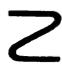
\includegraphics[keepaspectratio]{images/part001_c7194320.jpg}}

We note that, if M and N are any two closed vector subspaces in a Hausdorff topological vector space E, then \(M + N\) is not necessarily closed in E, * even if E is a Hilbert space * (cf.~IV, p.~64, exerc. 13, d)).

PROPOSITION 3. --- Let E be a topological vector space over a complete non-discrete valued division ring K. Let M be a closed vector subspace of finite codimension n in E. Then every subspace N that is an algebraic complement of M in E is also a topological complement.

In N, the set \(\{0\}\) is closed, since it is the intersection of N and the set M which is closed in E; thus N is Hausdorff. As E/M is also Hausdorff, the canonical mapping of N on E/M, which is linear and bijective, is bicontinuous (I, p.~14, cor. 2), from which the proposition follows.

COROLLARY. --- Let E and F be two topological vector spaces over a complete non-discrete valued division ring. If F is Hausdorff and of finite dimension, then every continuous linear mapping of E on F is a strict morphism.

Remark. --- The results of Nos 2, 3 are no longer valid when K is discrete. For example, let \(K_{1}\) be a non-discrete valued division ring and K be the discrete division ring obtained by endowing \(K_{1}\) with the improper absolute value on \(K_{1}\) . Then \(K_{1}\) is a topological vector space of dimension 1 over K, but it is not isomorphic to \(K_{s}\) . However, we can show that the results of Nos 2, 3 are valid even when K is discrete, provided that we impose on the topological vector spaces considered, the property of having a fundamental system of balanced neighbourhoods of 0 (i.e.~neighbourhoods V such that \(K.V = V\) ) (I, p.~27, exerc. 14); this condition (which is always satisfied when K is a non-discrete valued division ring cf.~I, p.~7, prop. 4) is not valid for all topological vector spaces over K as the preceding example shows.

\subsection{Locally compact topological vector spaces}

THEOREM 3. --- Let K be a complete non-discrete valued division ring. If E is a Hausdorff topological vector space over K, which is such that some neighbourhood V of 0 in E is precompact, then E is of finite dimension. If \(E \neq \{0\}\) , then both K and E are locally compact.

In proving the first assertion, we need consider only the case when E is complete; for E is an everywhere dense subspace of its completion \(\hat{E}\) , and the closure \(\overline{V}\) of V in \(\hat{E}\) is compact and is a neighbourhood of 0 in \(\hat{E}\) (GT, III, § 3.4, prop. 7).

We can suppose then that there is a compact neighbourhood V of 0 in E. Let \(\alpha \in \mathbf{K}\) be such that \(0 < |\alpha| < 1\) ; then there are finitely many points \(a_i \in \mathbf{V}\) such that

\[
\mathrm{V} \subset \bigcup_ {i} (a _ {i} + \alpha \mathrm{V}).
\]

Let M be the finite dimensional subspace of E generated by the \(a_{i}\) ; it is closed in E (I, p.~14, cor. 1). In the Hausdorff topological vector space E/M the canonical image of V is a compact neighbourhood W of 0, such that \(W \subset \alpha W\) ; hence \(\alpha^{-1} W \subset W\) , and, by induction on n, \(\alpha^{-n} W \subset W\) for every positive integer n.~As W is absorbent, we conclude that W = E/M; and thus E/M is compact. To complete the proof of the first assertion in the theorem, it is sufficient, therefore, to establish the following lemma.

Lemma 1. --- Any compact topological vector space E over a non-discrete valued division ring, is just the set \(\{0\}\) .

Since E is complete we can suppose K is complete (I, p.~6). If \(E \neq \{0\}\) then E contains a line that is closed in E (I, p.~14, cor. 1) and therefore compact. This line is isomorphic to \(K_{s}\) (I, p.~12, prop. 2) and hence K must be compact. Now the mapping \(\xi \mapsto |\xi|\) of K in R is continuous and thus the image of K must be bounded, on the other hand there exists \(\gamma \in K\) with \(|\gamma| > 1\) , and the set \(|\gamma^{n}| = |\gamma|^{n}\) , \(n \in N\) , is unbounded. This contradiction shows that \(E = \{0\}\) .

To prove the second assertion in the theorem, if \(E \neq \{0\}\) then from the first part of the theorem E is isomorphic to \(K_{s}^{n}\) with n \textgreater{} 0; now K is complete, hence so is E, and thus E is locally compact. But \(K_{s}\) is isomorphic to a line in E (I, p.~12, prop. 2) which is necessarily closed in E (I, p.~14, cor. 1); it follows that K is locally compact.

Remark. --- The result of th. 3 is no longer true if K is a discrete division ring as is shown by the example of R (with the usual topology) considered as a topological vector space over the discrete field Q.

\section{METRISABLE TOPOLOGICAL VECTOR SPACES}

\subsection{Neighbourhoods of 0 in a metrisable topological vector space}

We say that a topological vector space E is metrisable if its topology is metrisable. Relative to the structure of its additive group and of its topology, E is, therefore, a metrisable group (GT, IX, § 3.1).

We know that, for a topological group to be metrisable, it is necessary and sufficient that there exists an enumerable fundamental system of neighbourhoods of the neutral element e, whose intersection is the single element e (GT, IX, § 3.1, prop. 1).

Also we know that the uniform structure of a metrisable topological vector space E, can be defined by an invariant distance \(d(x, y) = |x - y|\) , where \(x \mapsto |x|\) is a continuous mapping of E in \(R_{+}\) which satisfies the conditions: 1) \(|-x| = |x|\) ; 2) \(|x + y| \leqslant |x| + |y|\) ; 3) the relation \(|x| = 0\) is equivalent to x = 0 (GT, IX, § 3.1, prop. 3).

We saw (GT, IX, § 3.1, prop. 2) how such a distance \(d\) could be defined using a decreasing sequence \((\mathbf{W}_n)\) of neighbourhoods of 0 in E, forming a fundamental system of neighbourhoods and such that \(\mathbf{W}_{n+1} + \mathbf{W}_{n+1} + \mathbf{W}_{n+1} \subset \mathbf{W}_n\) . When E is a metrisable vector space over a non-discrete valued division ring K, we can also suppose that the \(\mathbf{W}_n\) are balanced (I, p.~7, prop. 4); if we revert to the process of definition of \(d\) (loc. cit.) we can see that the relation \(|\lambda| \leqslant 1\) implies that \(|\lambda x| \leqslant |x|\) . Further the conditions (EVT \(_i\) ) and (EVT \(_ii\) ) of I, p.~2 imply both that \(|\lambda x_0|\) tends to 0 as \(\lambda\) tends to 0 in K for every \(x_0 \in \mathrm{E}\) , and that \(|\lambda_0 x|\) tends to 0 as \(|x|\) tends to 0 for every \(\lambda_0 \in \mathrm{K}\) . Conversely, if the function \(|x|\) possesses all the preceding properties and if \(\mathbf{W}_n\) is the set of \(x \in \mathrm{E}\) such that \(|x| \leqslant 2^{-n}\) , then the \(\mathbf{W}_n\) form a fundamental system of balanced neighbourhoods of 0 for a metrisable topology on E that is compatible with the vector space structure of E.

Remark. --- One of the most important classes of metrisable vector spaces are the normed spaces (I, p.~3). But it must be noted that there exist metrisable vector spaces whose topology cannot be defined by a norm (I, § 3, exerc. 1); we shall study important examples later.

\subsection{Properties of metrisable vector spaces}

Every vector subspace of a metrisable topological vector space E is metrisable; the same is true of every quotient space E/M of E by a closed vector subspace M (GT, IX, § 3.1, prop. 4). Every product of an enumerable family of metrisable topological vector spaces is metrisable (GT, IX, § 2.4, cor. 2). If \(K_{0}\) is a complete valued division ring, and K is a subdivision ring everywhere dense in \(K_{0}\) , the completion \(\hat{E}\) of a metrisable vector space E over K is a metrisable vector space over \(K_{0}\) (I, p.~6 and GT, IX, § 2, No.~1, prop. 1). Finally, if E is a metrisable vector space that is complete, then for every closed vector subspace M of E, the quotient space E/M is complete (GT, IX, § 3.1, prop. 4).

\subsection{Continuous linear functions in a metrisable vector space}

THEOREM 1 (Banach). --- Let E and F be two metrisable vector spaces over a non-discrete valued division ring K, and let u be a continuous linear mapping of E in F. Suppose that E is complete. Then the following conditions are equivalent :

\begin{enumerate}
\def\labelenumi{(\roman{enumi})}
\item
  \(u\) is a strict surjective morphism.
\item
  F is complete and \(u\) is surjective.
\item
  The image of \(u\) is not meagre in \(\mathbf{F}\) (GT, IX, § 5.2).
\item
  For every neighbourhood \(\mathbf{V}\) of 0 in \(\mathbf{E}\) , the set \(\overline{u(\mathbf{V})}\) is a neighbourhood of 0 in \(\mathbf{F}\) . Firstly (i) implies (ii), for let \(u\) be a strict surjective morphism and \(\mathbf{N}\) be the kernel of \(u\) . Then \(u\) induces an isomorphism of \(\mathrm{E/N}\) on \(\mathbf{F}\) . But \(\mathbf{E}\) is metrisable and complete, hence \(\mathrm{E/N}\) is complete (GT, IX, § 3.1, prop. 4), therefore \(\mathbf{F}\) is complete.
\end{enumerate}

Next (ii) implies (iii). Let F be complete and u be surjective. The image of u is precisely F and therefore not meagre in F from Baire's theorem (GT, IX, § 5.3).

The following lemma shows that (iii) implies (iv).

Lemma 1. --- Let E and F be two topological vector spaces over a non-discrete valued division ring K, and let u be a continuous linear mapping of E in F such that the image of E is not meagre. Then, for every neighbourhood V of 0 in E, the set \(\overline{u(V)}\) is a neighbourhood of 0 in F.

Let W be a balanced neighbourhood of 0 in E such that \(W + W \subset V\) (I, § 1.5, prop. 4). Let \(\alpha\) be an element of K such that \(|\alpha| > 1\) ; then E is the union of the sets \(\alpha^{n}W\) where n varies in N; in fact, for all \(x \in E\) , there exists \(\beta \in K\) such that \(x \in \beta W\) (I, p.~7, prop. 4) and there exists an integer \(n \geqslant 0\) such that \(|\beta| < |\alpha|^{n}\) , then \(x \in \alpha^{n}W\) since W is balanced. Hence, \(u(E)\) is the union of the sequence of sets \(u(\alpha^{n}W) = \alpha^{n}u(W)\) , and as \(u(E)\) is not meagre in F, one at least of the sets \(\alpha^{n}\overline{u(W)}\) possesses an interior point (GT, IX, § 5.3, def. 2) and therefore \(\overline{u(W)}\) has an interior point.

Let \(y_0\) be an interior point of \(\overline{u(\mathbf{W})}\) ; since \(-u(\mathbf{W}) = u(\mathbf{W})\) , and therefore \(-\overline{u(\mathbf{W})} = \overline{u(\mathbf{W})}\) it follows that \(0 = y_0 + (-y_0)\) is an interior point of \(\overline{u(\mathbf{W})} + \overline{u(\mathbf{W})}\) . As vector addition is a continuous mapping of \(F \times F\) in \(F\) , the set \(\overline{u(\mathbf{W})} + \overline{u(\mathbf{W})}\) is contained in the closure of the set

\[
u (\mathrm{W}) + u (\mathrm{W}) = u (\mathrm{W} + \mathrm{W}) \subset u (\mathrm{V});
\]

hence \(\overline{u(\mathrm{V})}\) is a neighbourhood of 0 in F.

Before proving that (iv) implies (i) we prove the following lemma, where we make the convention that, in all metric spaces, \(\mathbf{B}_{r}(x)\) denotes the closed ball of centre x and radius r.

Lemma 2. --- Let E and F be two metric spaces, and suppose that E is also complete. Let u be a linear mapping of E in F having the following property: whatever the number r \textgreater{} 0, there exists a number \(\rho(r) > 0\) such that, for all \(x \in E\) , we have

\[
\mathrm{B} _ {\rho (r)} (u (x)) \subset \overline {{u (\mathrm{B} _ {r} (x))}}.
\]

In these conditions, for all \(a > r\) , the image \(u(\mathbf{B}_a(x))\) contains the ball \(\mathbf{B}_{\rho(r)}(u(x))\) .

Let \((r_n)\) be an infinite sequence of numbers \(>0\) such that \(r_1 = r\) and \(a = \sum_{n=1}^{\infty} r_n\) . For each index \(n\) there exists a number \(\rho_n > 0\) (with \(\rho_1 = \rho(r)\) ) such that

\[
\mathrm{B} _ {\rho_ {n}} (u (x)) \subset \overline {{u (\mathrm{B} _ {r _ {n}} (x))}}
\]

for all \(x \in E\) ; we can, and will, suppose that \(\lim \rho_{n} = 0\) .

Let \(x_0\) be a point of \(E\) , and \(y\) be a point of \(B_{\rho(r)}(u(x_0))\) . We shall show that \(y\) belongs to \(u(B_a(x_0))\) .

For this, a sequence \((x_{n})_{n>0}\) of points of E is defined inductively such that, for all \(n \geqslant 1\) , we have \(x_{n} \in \mathbf{B}_{r_{n}}(x_{n-1})\) and \(u(x_{n}) \in \mathbf{B}_{\rho_{n+1}}(y)\) . If the \(x_{i}\) have been defined for \(0 \leqslant i \leqslant n - 1\) satisfying these relations, then we have \(y \in \mathbf{B}_{\rho_{n}}(u(x_{n-1}))\) ; since

\[
\mathrm{B} _ {\rho_ {n}} (u (x _ {n - 1})) \subset \overline {{u (\mathrm{B} _ {r _ {n}} (x _ {n - 1}))}},
\]

there exists a point \(x_{n} \in \mathbf{B}_{r_n}(x_{n-1})\) whose image \(u(x_{n})\) belongs to the neighbourhood \(\mathbf{B}_{\rho_{n+1}}(y)\) of \(y\) , which establishes the existence of the sequence \((x_{n})\) .

Since the distance of \(x_{n}\) from \(x_{n+p}\) is less than \(r_{n+1} + r_{n+2} + \cdots + r_{n+p}\) , which is arbitrarily small when n is large, the sequence \((x_{n})\) is a Cauchy sequence in E. As E is complete, the sequence \((x_{n})\) converges to a point x of E. The distance of \(x_{0}\) from x is less than \(\sum_{n=1}^{\infty} r_{n} = a\) , thus \(x \in \mathbf{B}_{a}(x_{0})\) . But u is continuous, thus the sequence \(u(x_{n})\) converges to \(u(x)\) ; also \(u(x_{n}) \in \mathbf{B}_{\rho_{n+1}}(y)\) , hence \(y = u(x)\) , and the lemma is proved.

We return to the theorem and show that (iv) implies (i). Suppose that \(u\) satisfies condition (iv). For each of the spaces E and F, consider a distance that is invariant under translation and defines its topology (I, p.~16). By hypothesis, the set \(u(\mathbf{B}_r(0))\) is a neighbourhood of 0 in F for every \(r > 0\) , and thus there exists a number \(\rho(r) > 0\) such that \(\mathbf{B}_{\rho(r)}(0) \subset u(\mathbf{B}_r(0))\) . By translation we conclude that \(\mathbf{B}_{\rho(r)}(u(x)) \subset u(\mathbf{B}_r(x))\) for all \(r > 0\) and all \(x \in E\) . From lemma 2, for every pair of real positive numbers \((a, r)\) , \(a > r > 0\) , we have \(\mathbf{B}_{\rho(r)}(0) \subset u(\mathbf{B}_a(0))\) ; thus \(u\) is a strict morphism of E on F. We have shown that (iv) implies (i) and the proof of the theorem is completed.

COROLLARY 1. --- If E and F are two complete metrisable vector spaces over a non-discrete valued division ring, then every bijective continuous linear mapping of E on F is an isomorphism.

In particular, if E and F are two complete normed spaces, there exists a number \(a > 0\) such that \(\| u(x)\| \geqslant a.\| x\|\) for all \(x\in \mathbf{E}\) .

COROLLARY 2. --- Let E be a vector space over a non-discrete valued division ring, let \(T_{1}\) and \(T_{2}\) be two topologies on E compatible with its vector space structure and for each of which E is metrisable and complete. Then, if \(T_{1}\) and \(T_{2}\) are comparable, they are identical.

COROLLARY 3. --- Let E and F be two complete metrisable vector spaces over a non-discrete valued division ring. In order that a continuous linear mapping u of E in F should be a strict morphism, it is necessary and sufficient that \(u(\mathrm{E})\) be closed in F.

The condition is necessary, because if u is a strict morphism, the image \(u(\mathrm{E})\) , being isomorphic to the quotient \(\mathrm{E}/u^{-1}(0)\) , is complete (I, p.~17) and therefore closed in F. The condition is sufficient, since, if \(u(\mathrm{E})\) is closed in F, then \(u(\mathrm{E})\) must be a complete metrisable vector space and thus by theorem 1 u is a strict morphism of E on \(u(\mathrm{E})\) .

COROLLARY 4. --- Let E be a complete metrisable vector space over a non-discrete valued division ring. If M and N are two closed vector subspaces, that are (algebraic) complements in E, then E is the direct topological sum of M and N.

For \(M \times N\) is a complete metrisable vector space and the mapping \((y, z) \mapsto y + z\) of \(M \times N\) on E is continuous and bijective, therefore an isomorphism (cor. 1).

COROLLARY 5 (The closed graph theorem). --- Let E and F be two complete metrisable vector spaces over a non-discrete valued division ring. In order that a linear mapping u of E in F be continuous, it is necessary and sufficient that its graph, in the product space \(E \times F\) , be closed.

The condition is necessary since the graph of a continuous mapping into a Hausdorff space is closed (GT, I, § 8.1, cor. 2). To see that it is sufficient, note that it implies that the graph G of u, which is a closed vector subspace of the complete metrisable space \(E \times F\) , is itself metrisable and complete. The projection \(z \mapsto \operatorname{pr}_{1}(z)\) of G on E is a bijective, continuous linear mapping, therefore an isomorphism (cor. 1); since its inverse mapping is \(x \mapsto (x, u(x))\) , it follows that \(u\) is continuous in E.

We can express this corollary in the following form: \(u\) is continuous if the following situation holds: if the sequence \((x_{n})\) of points of E both converges to 0 and is such that the sequence \((u(x_{n}))\) converges to \(y\) , then it is necessarily the case that \(y = 0\) .

Example. --- Let E be a vector subspace of the space of real-valued functions defined on I = \([0, 1]\) ; let \(\|f\|\) be a norm on E, under which E is complete, and such that its topology is finer than the topology of simple convergence. Suppose further that E contains the set \(\mathcal{C}^{\infty}(\mathrm{I})\) of functions infinitely differentiable on I; we shall show that there exists an integer \(k \geqslant 0\) , such that E contains the set \(\mathcal{C}^{k}(\mathrm{I})\) of all functions with a continuous k-th derivative in I.

For every pair of integers \(m > 0\) , \(n \geqslant 0\) , let \(V_{mn}\) be the set of functions \(f \in \mathcal{C}^{\infty}(\mathrm{I})\) such that \(|f^{(h)}(x)| \leqslant 1 / m\) for \(0 \leqslant h \leqslant n\) and for all \(x \in \mathrm{I}\) . The \(V_{m,n}\) form a fundamental system of neighbourhoods of 0 for a metrisable topology compatible with the vector space structure of \(\mathcal{C}^{\infty}(\mathrm{I})\) , further \(\mathcal{C}^{\infty}(\mathrm{I})\) is complete in this topology (FVR, II, p.~2, th. 1). Let \(u\) be the canonical mapping of \(\mathcal{C}^{\infty}(\mathrm{I})\) in E; we show that \(u\) is continuous. From cor. 5 above it is sufficient to prove that if a sequence \((f_n)\) converges to 0 in \(\mathcal{C}^{\infty}(\mathrm{I})\) and to a limit \(f\) in E then necessarily \(f = 0\) . But this is immediate since, by hypothesis, \(f\) is the simple convergence limit of \((f_n)\) . Hence there exists an integer \(k \geqslant 0\) and a number \(a > 0\) such that the relation

\[
p_{k}(f) = \sup_{\substack{x\in \mathbf{I}\\ 0\leqslant h\leqslant k}}\big|f^{(h)}(x)\big|\leqslant a
\]

implies \(\| f\| \leqslant 1\) for all \(f\in \mathcal{C}^{\infty}(\mathrm{I})\)

But \(p_k\) is a norm on the space \(\mathcal{C}^k(\mathrm{I})\) and \(\mathcal{C}^\infty(\mathrm{I})\) is a subspace that is everywhere dense in \(\mathcal{C}^k(\mathrm{I})\) for this norm (the set of polynomials being already everywhere dense in \(\mathcal{C}^k(\mathrm{I})\) , an immediate consequence of the Weierstrass-Stone theorem). By what has gone before, the identity mapping of \(\mathcal{C}^\infty(\mathrm{I})\) (carrying the norm \(p_k\) ) in \(\mathrm{E}\) , is continuous, and so it can be extended continuously to the whole space \(\mathcal{C}^k(\mathrm{I})\) (since \(\mathrm{E}\) is complete). This proves our assertion.

PROPOSITION 1. --- Let E, F be two topological vector spaces over a non-discrete valued division ring K. We suppose that :

\begin{enumerate}
\def\labelenumi{\arabic{enumi})}
\item
  E is metrisable and complete.
\item
  There exists a sequence \((\mathbf{F}_{n})\) of complete metrisable vector spaces over K and, for each n, an injective continuous linear mapping \(v_{n}\) of \(F_{n}\) in F such that F is the union of the subspaces \(v_{n}(\mathbf{F}_{n})\) .
\end{enumerate}

Then let u be a linear mapping of E in F. If the graph of u is closed in \(E \times F\) , then there exists an integer n and a continuous linear mapping \(u_{n}\) of E in \(F_{n}\) such that \(u = v_{n} \circ u_{n}\) (which implies that u is continuous and that \(u(\mathrm{E}) \subset v_{n}(\mathrm{F}_{n})\) ).

Let G be the graph of u in \(E \times F\) . For all n, we consider the continuous linear mapping \(w_{n}:(x,y)\mapsto(x,v_{n}(y))\) of \(E \times F_{n}\) in \(E \times F\) ; as G is closed, the set \(w_{n}^{-1}(\mathbf{G})=\mathbf{G}_{n}\) is a closed vector subspace of \(E \times F_{n}\) ; if \(p_{n}\) is the restriction to \(G_{n}\) of the first projection \(pr_{1}\) , we have \(p_{n}(\mathbf{G}_{n})=u^{-1}(v_{n}(\mathbf{F}_{n}))\) . As \(p_{n}\) is continuous and \(G_{n}\) is complete (since \(G_{n}\) is closed in the complete space \(E \times F_{n}\) ), \(p_{n}(\mathbf{G}_{n})\) is, by theorem 1, either meagre in E or it is the whole of E. But, by hypothesis, E is the union of the \(p_{n}(\mathbf{G}_{n})\) , and as E is complete, the \(p_{n}(\mathbf{G}_{n})\) cannot all be meagre in E by Baire's theorem (GT, IX, § 5.3, th. 1). Therefore there exists an integer n such that \(p_{n}(\mathbf{G}_{n}) = \mathbf{E}\) , or in other words \(u(\mathbf{E}) \subset v_{n}(\mathbf{F}_{n})\) . Further, as \(v_{n}\) is injective, \(G_{n}\) is the graph of a linear mapping \(u_{n}\) of E in \(F_{n}\) , and by the closed graph theorem (I, p.~19, cor. 5) \(u_{n}\) is continuous; it follows then from the definitions that \(u = v_{n} \circ u_{n}\) .

\exercisesheading

\exercisegroup

\begin{enumerate}
\def\labelenumi{\arabic{enumi})}
\item
  Let \(E_{0}=Q_{p}^{N}\) be the vector space over the p-adic field \(Q_{p}\) (GT, III, § 6, exerc. 23) which is the product of an enumerable infinity of factor each identical with \(Q_{p}\) . Let \(P\subset E_{0}\) be the set \(Z_{p}^{N}\) , and let E be the vector subspace of \(E_{0}\) generated by P. On the additive group P we consider the product compact topology of the topologies of the factors \(Z_{p}\) , and we denote by B the filter of neighbourhoods of 0 in P for this topology. Show that B is a fundamental system of neighbourhoods of 0 in E for a topology T compatible with the additive group structure of E, that satisfies \((\mathrm{EVT}_{\mathrm{I}}^{\prime})\) and \((\mathrm{EVT}_{\mathrm{III}}^{\prime})\) but not \((\mathrm{EVT}_{\mathrm{II}}^{\prime})\) (prove that the homothety \(x\mapsto x/p\) is not continuous in E).
\item
  Let K be a non-discrete topological division ring, \(K_{0}\) the division ring K with the discrete topology. The discrete topology on \(K_{0}\) is compatible with its additive group structure, and when we consider \(K_{0}\) as a vector space over K, it satisfies the axioms (EVT \(_{II}\) ) and (EVT \(_{III}\) ) but not (EVT \(_{I}\) ).
\item
  For every real number \(\alpha > 0\) , let \(G_{\alpha}\) be the topological group \(\mathbf{R} / \alpha \mathbf{Z}\) , and let \(G\) be the topological product group \(\prod_{\alpha} G_{\alpha}\) ( \(\alpha\) varying in the set of number \(>0\) ). For every \(x \in \mathbf{R}\) ,
\end{enumerate}

let \(t_{\alpha}(x)\) be the canonical image of \(x\) in \(G_{\alpha}\) ; the mapping \(\phi : x \to (t_{\alpha}(x))\) is a continuous injective homomorphism of \(\mathbf{R}\) in \(G\) . We consider on \(\mathbf{R}\) the topology that is the inverse image by \(\phi\) of that of \(G\) , and denote by \(E\) the topological group formed by \(\mathbf{R}\) with this topology. Show that when \(E\) is considered as a vector space over \(\mathbf{R}\) its topology satisfies \((\mathrm{EVT}_{I}^{\prime})\) and \((\mathrm{EVT}_{II}^{\prime})\) but not \((\mathrm{EVT}_{III}^{\prime})\) .

\begin{enumerate}
\def\labelenumi{\arabic{enumi})}
\setcounter{enumi}{3}
\item
  Let E be a vector space over a division ring K with a valuation; we suppose that E carries a metrisable topology compatible with its additive group structure. Suppose further that this topology satisfies axioms (EVT \(_{I}\) ) and (EVT \(_{II}\) ); show that if one of the two metrisable groups K, E is complete then the topology also satisfies (EVT \(_{III}\) ) and is, in consequence, compatible with the vector space structure of E (cf.~GT, IX, § 5, exerc. 23).
\item
  Let \(\mathbf{K}\) be a non-discrete valued field, and \(S\) be an arbitrary infinite set.
\end{enumerate}

\begin{enumerate}
\def\labelenumi{\alph{enumi})}
\item
  Let \(\mathbf{D} = (a_n)\) be an enumerable infinity of elements of \(\mathbf{S}\) . For every \(\lambda \in \mathbf{K}\) such that \(|\lambda| \leqslant 1\) , let \(u_{\lambda}\) be the element of the normed space \(\mathcal{B}_{\mathbf{K}}(\mathbf{S})\) , (I, p.~4, Example) of bounded mappings of \(\mathbf{S}\) in \(\mathbf{K}\) , such that \(u_{\lambda}(a_n) = \lambda^n\) for all \(n \in \mathbf{N}\) and \(u_{\lambda}(b) = 0\) for \(b \notin \mathbf{D}\) . Show that the family \((u_{\lambda})\) is algebraically independent.
\item
  Deduce that every basis of the vector space \(\mathcal{B}_{\mathbf{K}}(\mathbf{S})\) has the same cardinality as \(\mathrm{K}^{\mathrm{s}}\) (using \(a\) ) show that the cardinal of every basis of \(\mathcal{B}_{\mathbf{K}}(\mathbf{S})\) is at least equal to Card (K); note on the other hand that \(\operatorname{Card}(\mathcal{B}_{\mathbf{K}}(\mathbf{S})) = \operatorname{Card}(\mathbf{K}^{\mathrm{s}})\) and use A, II, § 2, exerc. 22).
\item
  Show in the same way that every basis of the vector space \(\ell_{\mathbf{K}}^{1}(\mathbf{S})\) has the cardinality of \((\mathbf{K}\times \mathbf{S})^{\mathbf{N}}\) .
\end{enumerate}

\begin{enumerate}
\def\labelenumi{\arabic{enumi})}
\setcounter{enumi}{5}
\tightlist
\item
  Let \(\mathbf{K}\) be a non-discrete valued division ring. Show that, for the space \(\ell_{\mathbf{K}}^{1}(\mathbf{N})\) of absolutely summable sequences \(x = (\xi_n)\) of elements of \(\mathbf{K}\) , the norms \(\| x \|_1 = \sum_{n=0}^{\infty} |\xi_n|\) and \(\| x \| = \sup_n |\xi_n|\) are not equivalent (cf.~GT, IX, § 3.3, prop. 7); show that \(\ell_{\mathbf{K}}^{1}(\mathbf{N})\) with the norm \(\| x \|\) is never complete even if \(\mathbf{K}\) is complete; what is its closure in \(\mathcal{B}_{\mathbf{K}}(\mathbf{N})\) ?
\end{enumerate}

¶ 7) * Let A be a ring with a discrete valuation, v the normed valuation of the division ring of fractions K of A; take the absolute value \(a^{v}\) on K, where 0 \textless{} a \textless{} 1. Let E be a normed vector space over K, for which the norm satisfies the ultrametric inequality

\[
\| x + y \| \leqslant \sup (\| x \|, \| y \|).
\]

\begin{enumerate}
\def\labelenumi{\alph{enumi})}
\item
  Denote by M the set of those \(x \in E\) for which \(\| x \| \leqslant 1\) , and by \(\pi\) a uniformizer of A; M is an A-module, and \(M / \pi M\) a vector space on the residual division ring \(k = A / \pi A\) of A. Let \((e_{\lambda})_{\lambda \in L}\) be a family of elements of M such that the images of \(e_{\lambda}\) in \(M / \pi M\) form a basis of this vector \(k\) -space. Show that \((e_{\lambda})\) is an independent family in E and that the vector subspace F of E generated by \((e_{\lambda})\) is dense in E.
\item
  If we put \(\| x\| _1 = \sup_{\lambda}|\xi_\lambda |,\) for every \(x = \sum_{\lambda}\xi_{\lambda}e_{\lambda}\) in F, show that on F the norms \(\| x\|\) and \(\| x\| _1\) are equivalent.
\item
  Let \(\mathbf{K}\) be complete. Deduce from \(a)\) and \(b)\) that, if \(\mathbf{L}\) is finite, the completion \(\hat{\mathbf{E}}\) of \(\mathbf{E}\) is isomorphic to \(\mathbf{K}^{\mathrm{L}}\) ; if \(\mathbf{L}\) is infinite \(\hat{\mathbf{E}}\) is isomorphic to the subspace \(\mathcal{C}_{\mathbf{K}}^{0}(\mathbf{L})\) of \(\mathcal{B}_{\mathbf{K}}(\mathbf{L})\) formed of the families \((\xi_{\lambda})\) such that \(\lim \xi_{\lambda} = 0\) for the filter of complements of finite subsets of \(\mathbf{L}\) .
\item
  We suppose K and E complete; let G be a second normed complete space over K whose norm satisfies the ultrametric inequality. Show that on replacing (if necessary) the norm of \(\mathcal{L}(\mathrm{E};\mathrm{G})\) (GT, X, § 3.2) by an equivalent one, then \(\mathcal{L}(\mathrm{E};\mathrm{G})\) is isometric to the vector space of families \((y_{\lambda})_{\lambda \in L}\) of elements of G such that \(\sup_{\lambda \in L}\| y_{\lambda}\| < +\infty\) , carrying the norm \(\sup_{\lambda \in L}\| y_{\lambda}\|\) (which is also an ultrametric norm).
\end{enumerate}

\begin{enumerate}
\def\labelenumi{\arabic{enumi})}
\setcounter{enumi}{7}
\item
  Let E be a topological vector space over a non-discrete topological division ring K. In order that there should exist a neighbourhood of the point \((0,0)\) in \(K \times E\) such that the mapping \((\lambda, x) \mapsto \lambda x\) should be uniformly continuous in this neighbourhood, it is necessary and sufficient that there exist a neighbourhood \(V_{0}\) of 0 in E such that the sets \(\lambda V_{0}\) form a fundamental system of neighbourhoods of 0 in E, where \(\lambda\) varies in the set of elements \(\neq 0\) of K. When K is a division ring with a non-discrete valuation and E is Hausdorff, show that the uniform structure of E is then metrisable.
\item
  Generalize prop. 5 of I, p.~8, to the case where the spaces \(\mathrm{E}_i\) ( \(\leqslant i \leqslant n\) ) and \(\mathrm{F}\) are topological vector spaces over an arbitrary non-discrete topological field.
\item
  Let E be a complete Hausdorff topological vector space over a non-discrete valued division ring K. Denote by F a vector subspace of E, and by T the topology on F induced by the topology \(T'\) of E; let B be a fundamental system of closed, balanced neighbourhoods of 0 for the topology T. Let \(F_{0}\) be the vector subspace of E, generated by the closures \(\overline{V}\) in E (relative to \(T'\) ) of the sets \(V \in B\) ; the sets \(\overline{V}\) form a fundamental system of neighbourhoods of 0 for a topology \(T_{0}\) on \(F_{0}\) , compatible with the vector space structure of \(F_{0}\) ; for this topology, \(F_{0}\) is complete, and the topology induced by \(T_{0}\) on F is identical with T.
\item
  In a topological vector space E over a non-discrete topological division ring K there exists a fundamental system B of closed neighbourhoods of 0, satisfying the conditions (EV \(_{II}\) ) and (EV \(_{III}\) ) as well as the two following :
\end{enumerate}

\((\mathrm{EV}_{\mathrm{Ia}})\) For each \(\mathbf{V} \in \mathfrak{B}\) , there exists \(\mathbf{W} \in \mathfrak{B}\) and a neighbourhood \(\mathbf{U}\) of 0 in \(\mathbf{K}\) such that \(\mathrm{UW} \subset \mathrm{V}\) . \((\mathrm{EV}_{\mathrm{Ib}})\) For every \(x \in \mathbf{E}\) and every \(\mathbf{V} \in \mathfrak{B}\) , there exists \(\lambda \neq 0\) in \(\mathbf{K}\) such that \(\lambda x \in \mathbf{V}\) . Conversely, let \(\mathbf{E}\) be a vector space over \(\mathbf{K}\) and let \(\mathfrak{B}\) be a filter base on \(\mathbf{E}\) satisfying the conditions \((\mathrm{EV}_{\mathrm{Ia}}), (\mathrm{EV}_{\mathrm{Ib}}), (\mathrm{EV}_{\mathrm{II}})\) and \((\mathrm{EV}_{\mathrm{III}})\) . Show that there is a topology on \(\mathbf{E}\) (and one such only), that is compatible with the vector space structure of \(\mathbf{E}\) , and for which \(\mathfrak{B}\) is a fundamental system of neighbourhoods of 0.

\begin{enumerate}
\def\labelenumi{\arabic{enumi})}
\setcounter{enumi}{11}
\item
  Let K be a discrete field, E the division ring of fractions of the ring of formal series A = K{[}{[}X, Y{]}{]} in two indeterminate variables on K (A, IV, p.~36). For every \(n \geqslant 0\) , let \(V_{n} \subset A\) be the set of formal series of total degree at least equal to n.~Show that in E, the sets \(V_{n}\) form a fundamental system of neighbourhoods of 0, for a topology compatible with the vector space structure of E (over K), for which E is metrisable and complete; if further K is a finite field, then E is locally compact. Show that the K-bilinear mapping \((u, v) \mapsto uv\) of E × E in E is continuous at the point \((0, 0)\) but that there exists \(u_{0} \in E\) such that \(v \mapsto u_{0}v\) is not continuous in E (for example \(u_{0} = 1/X\) ).
\item
  Let E be a vector space of infinite dimension over R, and let T be the family of all absorbent and balanced sets of E. Show that T does not satisfy axiom \((\mathrm{EV}_{\mathrm{III}})\) (in other words is not a fundamental system of neighbourhoods of 0 for a topology compatible with the additive group structure of E). For this, consider an infinite independent family \((e_{n})_{n\geqslant1}\) in E; for every integer \(n\geqslant1\) , let \(A_{n}\) be the set of points \(\sum_{i=1}^{n}t_{i}e_{i}\) such that \(|t_{i}|\leqslant1/n\) for \(1\leqslant i\leqslant n\) ; let A be the union of the \(A_{n}\) , and V be a subspace complementary to the subspace of E generated by the \(e_{n}\) , and write C for the set \(A+V\) ; show that there exists no set \(M\in T\) such that \(M+M\subset C\) .
\end{enumerate}

¶ 14) Let K be a Hausdorff topological division ring, \((E_{t})_{t\in I}\) an infinite family of Hausdorff topological vector spaces on K, none of which is the single point 0. We consider on \(F = \prod_{t\in I} E_t\) the topology \(\mathcal{T}\) , compatible with the additive group structure of \(F\) , for which a fundamental system of neighbourhoods of 0 is formed by the products \(\prod_{\iota \in I} V_{\iota}\) , where, for each \(\iota \in I\) , the set \(V_{t}\) is a neighbourhood of 0 in E (this topology is strictly finer than the product topology; cf.~GT, III, § 2, exerc. 23). We denote by \(T_{0}\) the topology induced by T on the subspace \(E = \bigoplus_{i \in I} E_{i}\) of F; E is closed in F for the topology T, and if each of the \(E_{t}\) is complete, then F is complete for the topology T, therefore E is complete for the topology \(T_{0}\) (GT, III, § 3, exerc. 10).

\begin{enumerate}
\def\labelenumi{\alph{enumi})}
\item
  Show that if there exists in K a neighbourhood of 0 bounded on the right (GT, III, § 6, exerc. 12) (in particular if K is a division ring with a valuation), the topology \(\mathcal{T}_0\) is compatible with the vector space structure of E. If, further, K is not discrete, then E is not a Baire space for any topology that is finer than \(\mathcal{T}_0\) and compatible with the vector space structure of E. b) Moreover, if there does not exist in K any neighbourhood of 0 bounded on the right (see c)) give an example of a family \((\mathrm{E}_t)\) such that the topology \(\mathcal{T}_0\) is not compatible with the vector space structure of E.
\item
  Let \(\mathbf{A} = \mathbf{R}[\mathbf{X}]\) be the ring of polynomials in one variable on \(\mathbf{R}\) . For every sequence \(s = (\varepsilon_n)_{n\geqslant 0}\) of real numbers \(>0\) , denote by \(\mathrm{V}_s\) the set of polynomials \(\sum_k a_k\mathrm{X}^k\in \mathrm{A}\) such that \(|a_k| < \varepsilon_k\) for all k. Let T be the set of the \(V_{s}\) where s varies in the set of sequences of numbers \textgreater0. Show that T is a fundamental system of symmetric neighbourhoods of 0 for a topology compatible with the ring structure of A. Let \(\mathbf{K} = \mathbf{R}(\mathbf{X})\) be the division ring of fractions of A; denote by S the family of subsets of K of the form \(\mathrm{U}(1 + \mathrm{U})^{-1}\) , where U varies in the set of the \(V_{s}\) not containing 1; show that S is a fundamental system of neighbourhoods of 0 for a topology compatible with the division ring structure of K, and that there does not exist in K any neighbourhood of 0 that is bounded.
\end{enumerate}

\(d\) ) For every Hausdorff topological division ring \(\mathbf{K}\) , show that there exists a set I such that on \(\mathbf{F} = \mathbf{K}^{\mathrm{I}}\) , the topology \(\mathcal{T}\) , defined above, is not compatible with the vector space structure of F.
